Agile programming

Testing specifics

\begin{figure}[H]
    \centering
    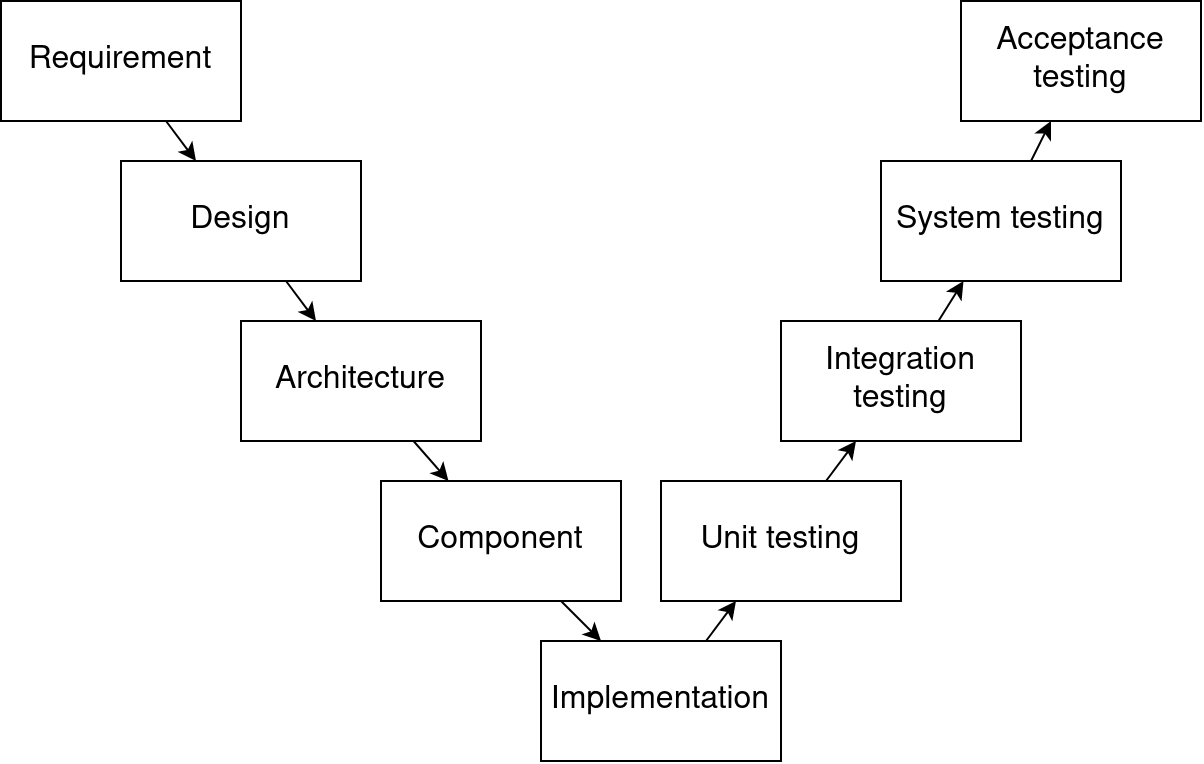
\includegraphics[width=0.5\textheight]{img/introduction/software-testing-v.drawio}
    \caption{Levels of abstraction and their corresponding tests}
    \label{fig:levels-of-abstraction-and-tests}
\end{figure}

Automated tests address the first issue.
Testing is well established and understood in software development.
In figure~\ref{fig:levels-of-abstraction-and-tests}, different types of tests can be seen that correspond to different levels of abstraction of the system.
Single components are unit tested in isolation, while their interaction is tested using integration tests and so on and so forth.
In order to validate code before an automatic integration occurs, a well-founded set of tests is needed.
Not only on the lowest levels, but also on the highest level, which is acceptance testing.
Without strong test suits,  faulty code may be integrated into a system and delivered to stakeholders.

Questions

\textit{Q1}: How can the setup and maintenance of an environment for higher level tests be abstracted and made accessible?
\textit{Q2}: How can multiple distribution systems be integrated into an automatic pipeline using a common base of data and metadata.